 

\documentclass[12pt]{article}
%%%%%%%%%%%%%%%%%%%%%%%%%%%%%%%%%%%%%%%%%%%%%%%%%%%%%%%%%%%%%%%%%%%%%%%%%%%%%%%%%%%%%%%%%%%%%%%%%%%%%%%%%%%%%%%%%%%%%%%%%%%%%%%%%%%%%%%%%%%%%%%%%%%%%%%%%%%%%%%%%%%%%%%%%%%%%%%%%%%%%%%%%%%%%%%%%%%%%%%%%%%%%%%%%%%%%%%%%%%%%%%%%%%%%%%%%%%%%%%%%%%%%%%%%%%%
\usepackage{amsfonts}
\usepackage{eurosym}
\usepackage{geometry}
\usepackage{amsmath,amsthm,amssymb}
\usepackage{graphicx}
\usepackage{comment}
\usepackage{adjustbox}
\usepackage{array}
\usepackage{multirow}
\usepackage{subcaption}
\usepackage{pifont}
\usepackage{amssymb}
\usepackage{comment}
\usepackage[utf8]{inputenc}
\usepackage{setspace}
\usepackage[hang, flushmargin, bottom]{footmisc}
%\usepackage[backend=biber,style=apa,url=false,isbn=false, extra = false]{biblatex}

%\addbibresource{references.bib}
\usepackage{footnotebackref}
\usepackage{xcolor}
\usepackage{hyperref}
\usepackage{booktabs}
\usepackage{pifont}
\usepackage{caption}
\usepackage{float}


\setlength{\textfloatsep}{5pt}
\captionsetup{font=normalsize}
\newcommand{\cmark}{\ding{51}}
\def\sym#1{\ifmmode^{#1}\else\(^{#1}\)\fi}
\renewcommand{\thetable}{\Roman{table}}
\geometry{verbose,tmargin=.5in,bmargin=.7in,lmargin=.7in,rmargin=.7in,nomarginpar}
\makeatletter

\begin{document}




\title{Meeting 24th of june}

\maketitle

In this document I will present what we are learnign from out empirical work. 

Before presenting our results it is important to clarify the sample selection criteria. We always first store the file without the sampling selection and then a second file with the sample selection. 

\begin{enumerate}
    \item We use the data in "1.solicitudes" to obtain the savings, age and other buyer characteristics. We store two files "1\_solicitudes" with all the requests and then another "1\_solicitudes\_yytoyyRV" with initial and final years and only the requests for annuities. 

    \item I use the data in "2.ofertas" \textcolor{red}{CURRENTLY WORKING ON BEING ABLE TO USE THE WHOLE DATA AND NOT ONLY THE REDUCED SAMPLE}
    
    The file '2\_ofertas\_muestra\_sol' contains a sample of offers for which requests were made, but it is not useful, because some of the requests lead to no offers or to offers that were not accepted. Hence we only use the file '2\_ofertas\_muestra\_acep'. 

    In the file '2\_ofertas\_muestra\_acep' we do the following sample selection: 1) kept only 'cod\_modalidad\_pension == 1' which are \textit{RV inmediata} 


    \item \textbf{Aceptaciones} just dropped sec\_beneficiario and kept one obs. per id\_certificado\_saldo because there was one per sec\_beneficiario. 
    \textcolor{red}{NOT CLEAR WHAT SEC\_BENEFICIARIO MEANS}

    \item \textbf{Clasificacion de riesgo} no sample selection

    \item[5.] In beneficiarios we do not do any sample selection. 
\end{enumerate}



For our main analysis we use the following sample selection criteria: 

Our sample consists on 8176 individuals and 497,000 offers, hence indiiduals receive on average 61 annuities offers. This offers differ on the number of guaranteed months and the withdrawal amount (ELD: excedente de libre disposicion). Hence we restrict our sample to offers with 0 guaranteed months and 0 ELD. Then the average individual receives 13 offers. 


\begin{tabular}{l*{5}{c}}
\hline\hline
            &       stats&            &            &            &            \\
            &          c1&          c2&          c3&          c4&          c5\\
\hline
r1          &        8176&      497045&    60.79318&      111577&    13.64689\\
\hline\hline
\end{tabular}






\section{IE 0}

Figure \ref{fig:ie0_0} shows the increase of requests over time. The increase is smooth with the exception of the year 2009 to 2010 that almost doubles. Probably there was a regulatory change. 
On average consumers make 10.5 requests for different financial products. 

CHECK WHY THE INCREASE IS SO BIG FROM 2009 TO 2010.

Important to note that individuals 
\begin{figure}[H]
\caption{}
\label{fig:ie0_0}
\centering{}%
\begin{tabular}{cc}
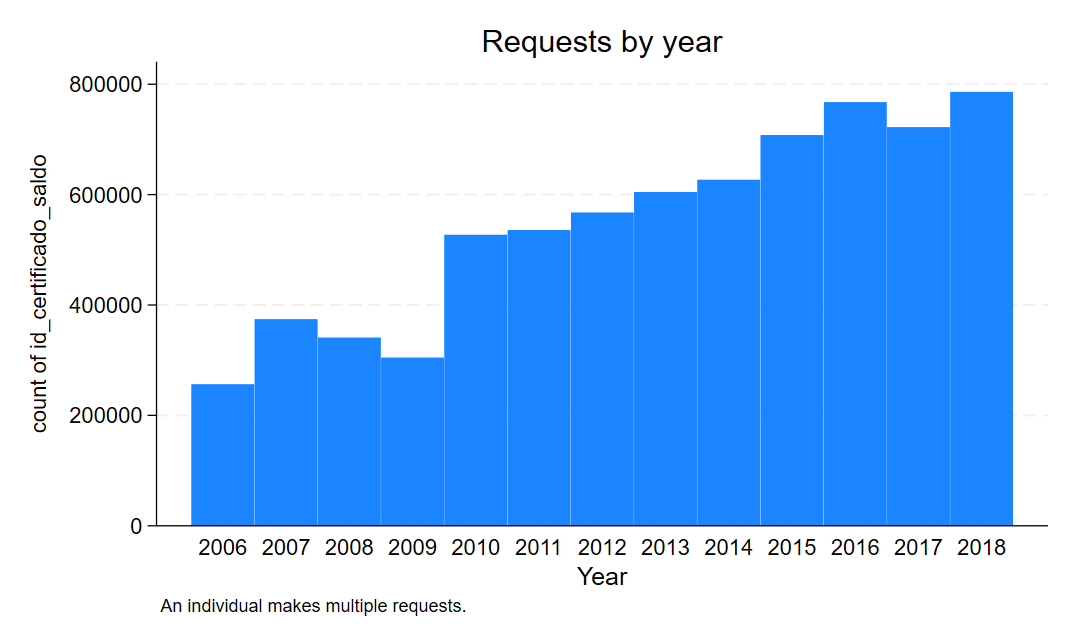
\includegraphics[scale=0.27]{figures/IE0_plot0.png}
\end{tabular}
\end{figure}


Figure \ref{fig:ie0_1} shows the amount of savings of individuals in the sample. Where 1UF is around 40 USD. The distribution is truncated at the 99th percentile of savings. 


\begin{figure}[H]
\caption{}
\label{fig:ie0_1}
\centering{}%
\begin{tabular}{cc}
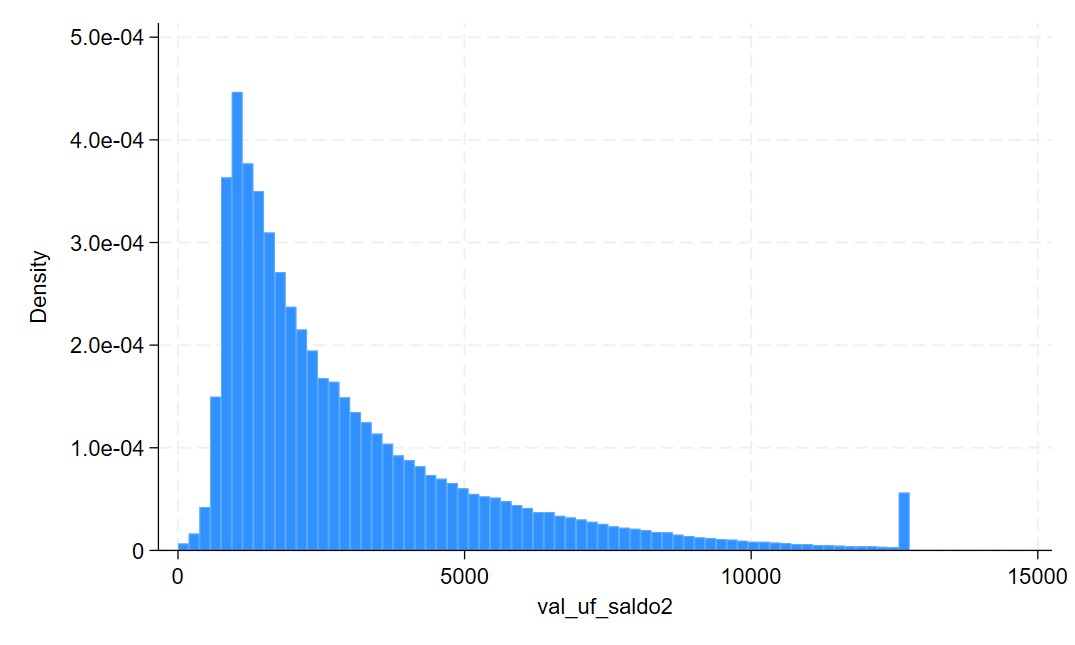
\includegraphics[scale=0.27]{figures/IE0_plot1.png} 
\end{tabular}
\end{figure}



Figure \ref{fig:ie0_2} shows the number of requests for each type of financial product in absolute terms and then their respective shares. The changes are not particularly large, it seems like the share of each financial product is relatively stable over time.

NOTE: ANNUITIES WITH PW(GREEN) START FROM 0 IN 2006 HENCE PROBABLY THEY ARE A FINANCIAL INNOVATION. 

\begin{figure}[H]
\caption{}
 \label{fig:ie0_2and3}
\centering{}%
\begin{tabular}{cc}
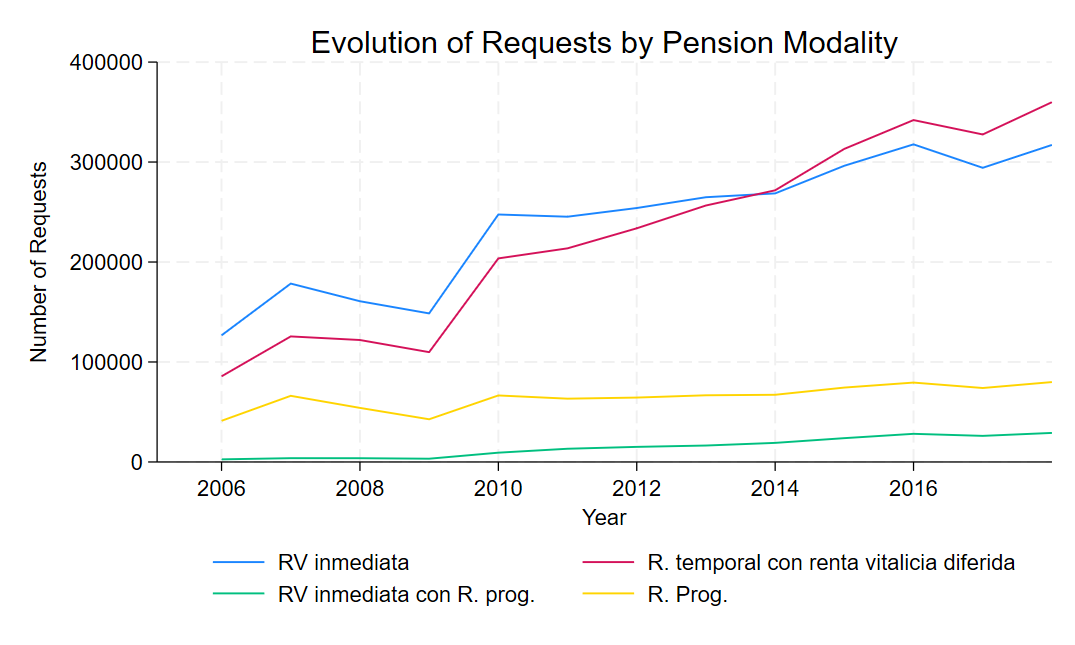
\includegraphics[scale=0.27]{figures/IE0_plot2.png} & 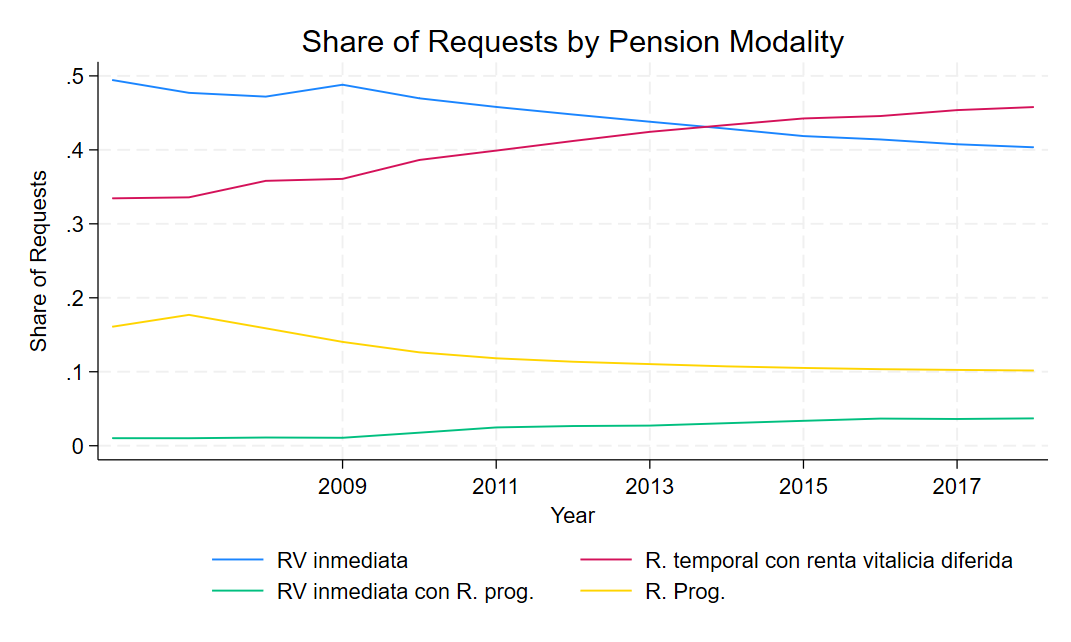
\includegraphics[scale=0.27]{figures/IE0_plot3.png}
\end{tabular}
\end{figure}


Figure \ref{fig:ie0_4} shows the shares for the whole sample as a function of savings. Richer individuals tend to buy more annuities with PW and less PW. This is explained by the fact that there is a minimum amount of savings required to buy an annuity and also could have to do with a higher life expectancy. 


\begin{figure}[H] 
\caption{}
\label{fig:ie0_4}
\centering{}%
\begin{tabular}{cc}
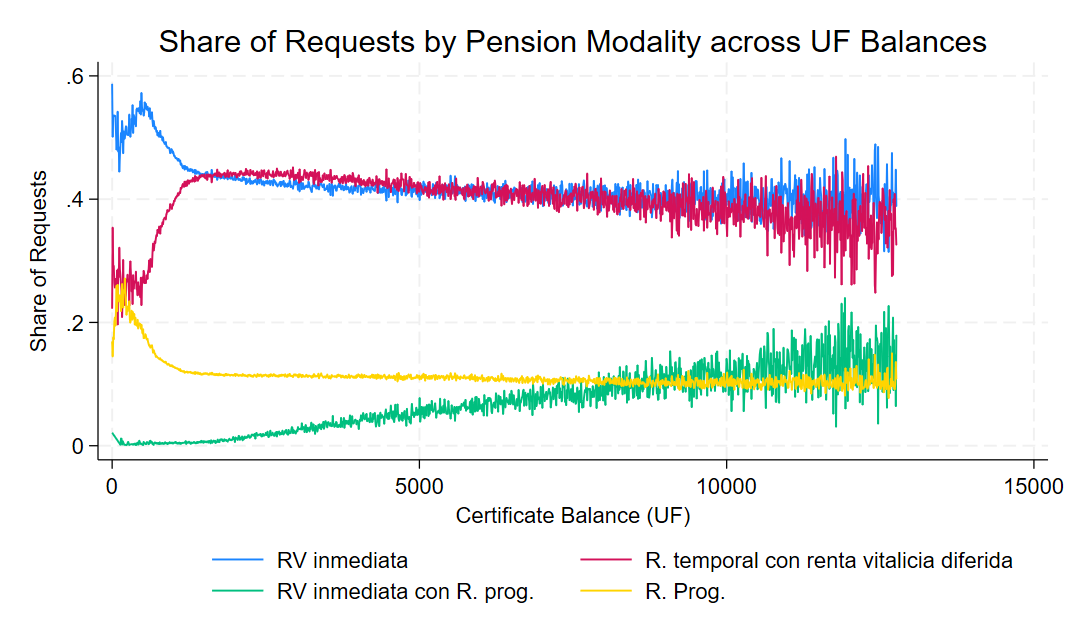
\includegraphics[scale=0.27]{figures/IE0_plot4.png}
\end{tabular}
\end{figure}

Figure \ref{fig:ie0_5} shows how many guaranteed months people buy. 
\begin{figure}[H] 
\caption{}
\label{fig:ie0_5}
\centering{}%
\begin{tabular}{cc}
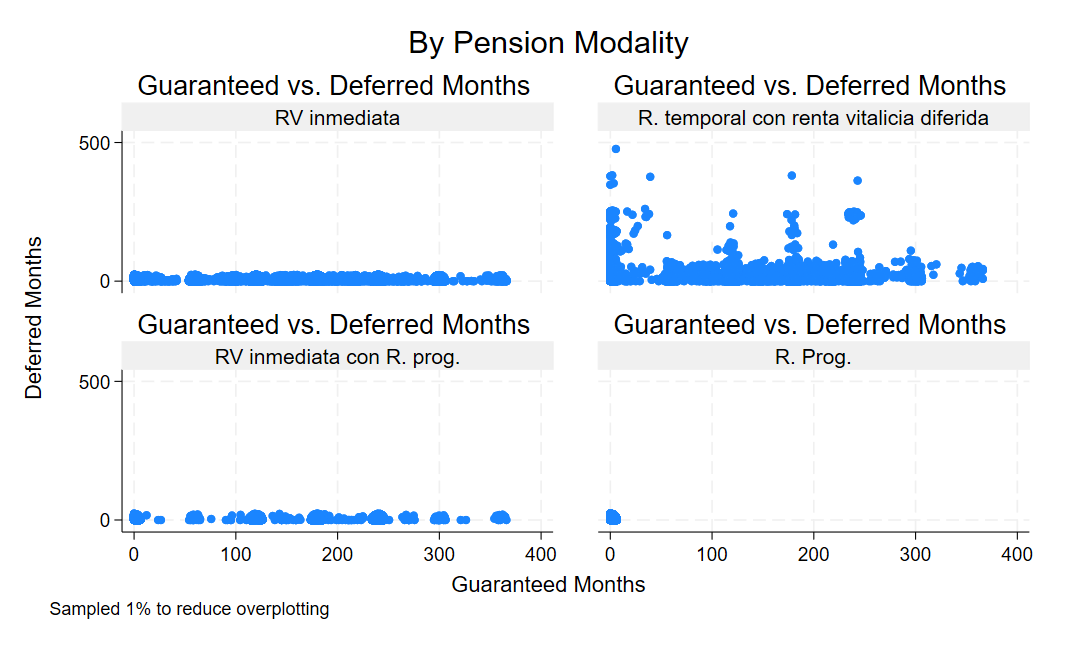
\includegraphics[scale=0.27]{figures/IE0_plot5.png}
\end{tabular}
\end{figure}

\section{IE 1}


Figure \ref{fig:ie1_1} the history of the credit rating for selected insurers.  
\begin{figure}[H]
\caption{}
 \label{fig:ie1_1}
\centering{}%
\begin{tabular}{cc}
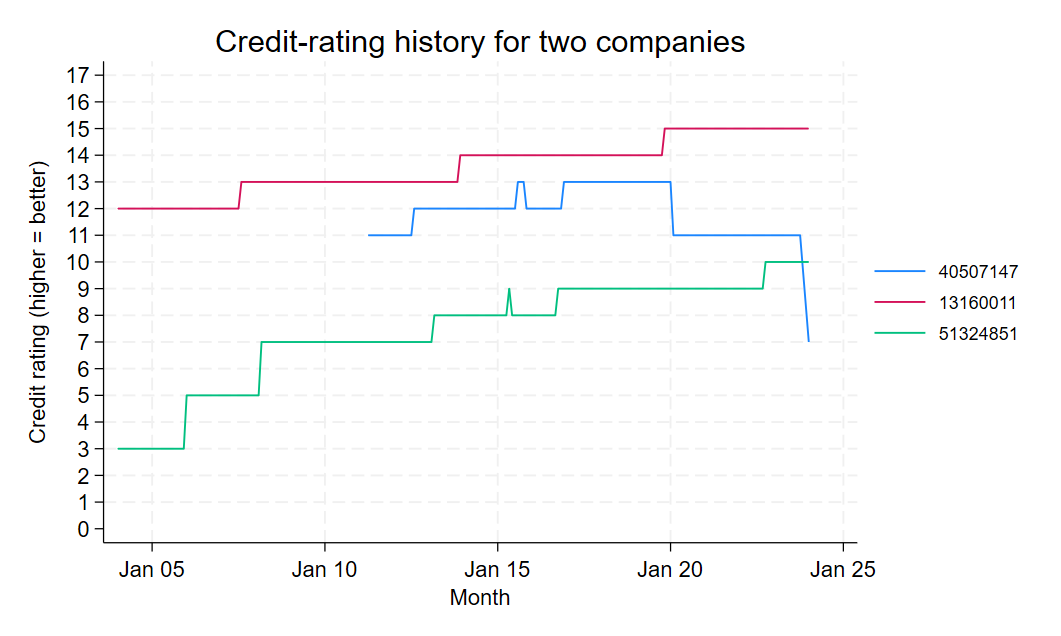
\includegraphics[scale=0.27]{figures/IE1_credit_history.png}
\end{tabular}
\end{figure}

Only 2\% of the offers constitute external offers, because individuals request offers from many financial products (make many requests), then receive many offers (one for each offering company) for each request, and then in case of requesting external offers they do it for only a subset of the initial offers. 

\section{IE1b}

This code just takes all the data of the offers (not only a sample) and creates .dta files where each of them contains a chunck of the data. Then filters the files to keep only the annuities and some years and finally joins all this filtered files into one big file with the offers. 


\section{IE 2}

Figure \ref{fig:ie2_0} shows the number of external offers that buyers request and figure \ref{fig:ie2_1} shows the distribution disaggregated by year. 

\begin{figure}[H]
\caption{}
\label{fig:ie2_0}
\centering{}%
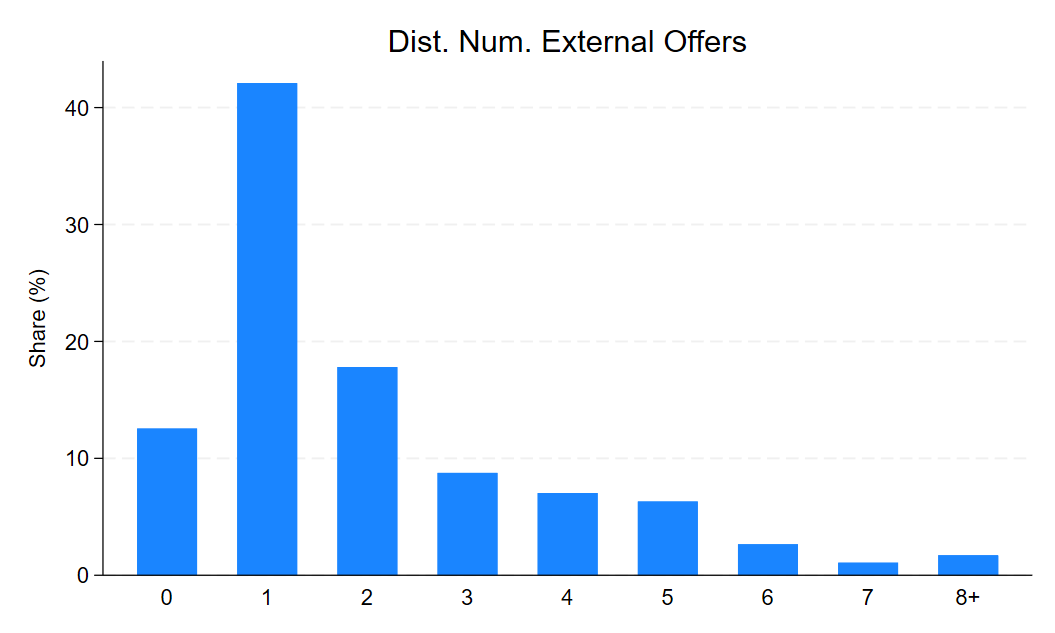
\includegraphics[scale=0.27]{figures/IE2_dist_external_offers.png}
\end{figure}


\begin{figure}[H]
\caption{}
\label{fig:ie2_1}
\centering{}%
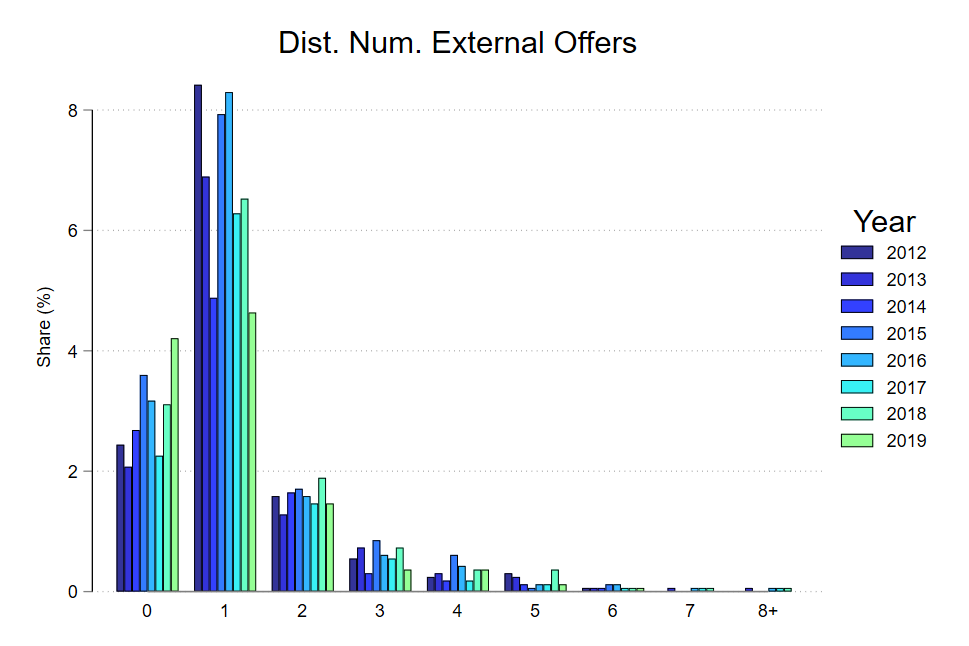
\includegraphics[scale=0.27]{figures/IE2_dist_external_offers_byyear.png}
\end{figure}






Figure \ref{fig:ie2_2} shows 


\begin{figure}[H]
\caption{}
 \label{fig:ie2_2}
\centering{}%
\begin{tabular}{cc}
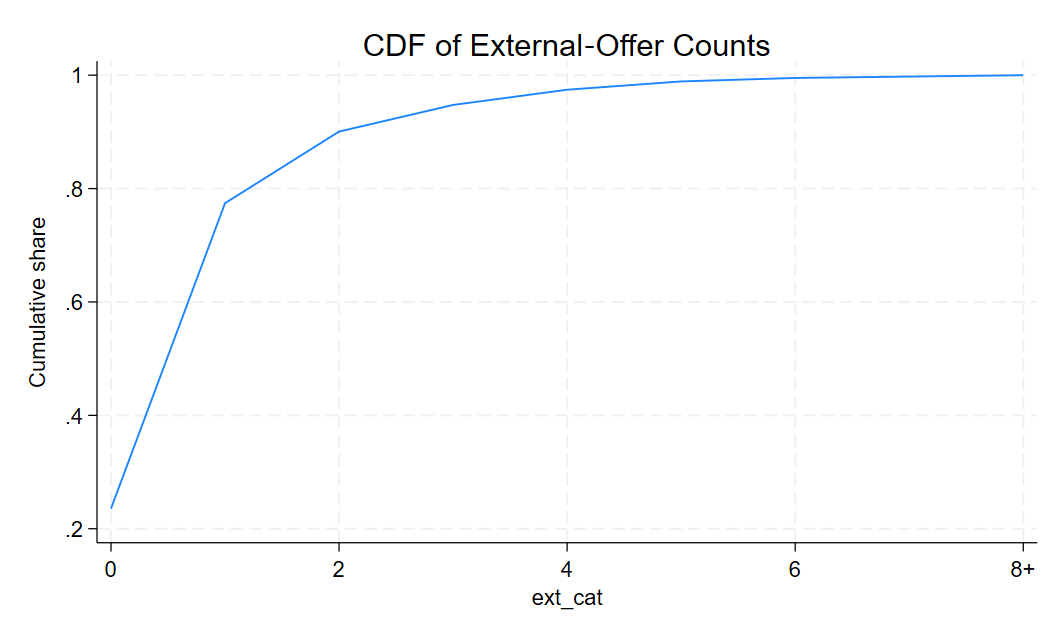
\includegraphics[scale=0.27]{figures/IE2_CDF_number_extoffers.png} &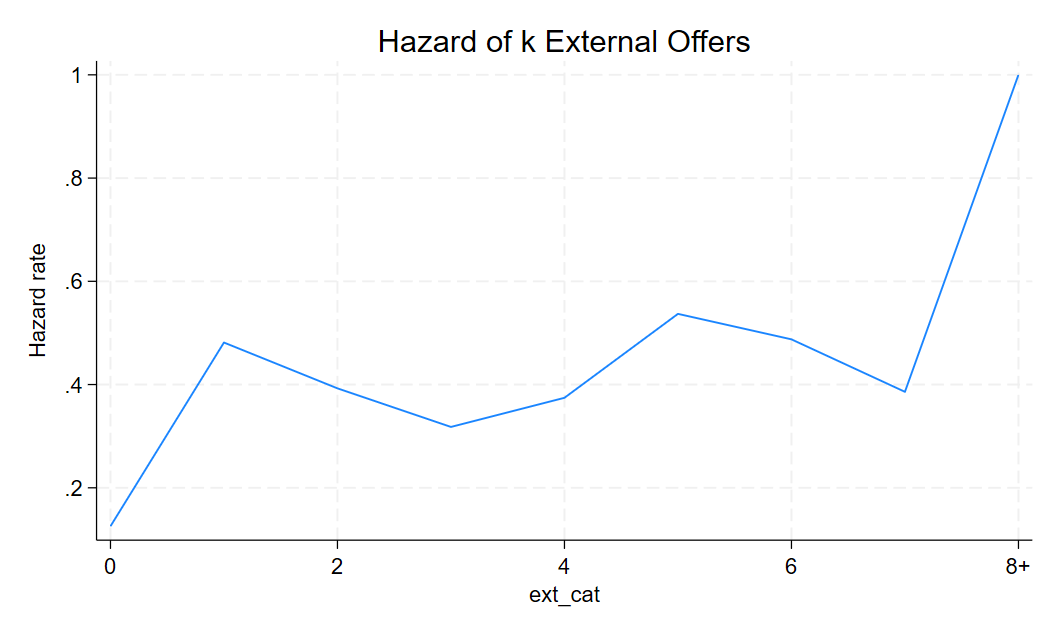
\includegraphics[scale=0.27]{figures/IE2_hazard_number_extoffers.png}
\end{tabular}
\end{figure}



Figure \ref{fig:ie2_3} shows the average number of searches for individuals grouped by their quintile of savings, which is a proxy of income. Specifically an increase of savings by a standard deviation is related to .72 additional searches. 


\begin{figure}[H]
\caption{}
\label{fig:ie2_3}
\centering{}%
\begin{tabular}{cc}
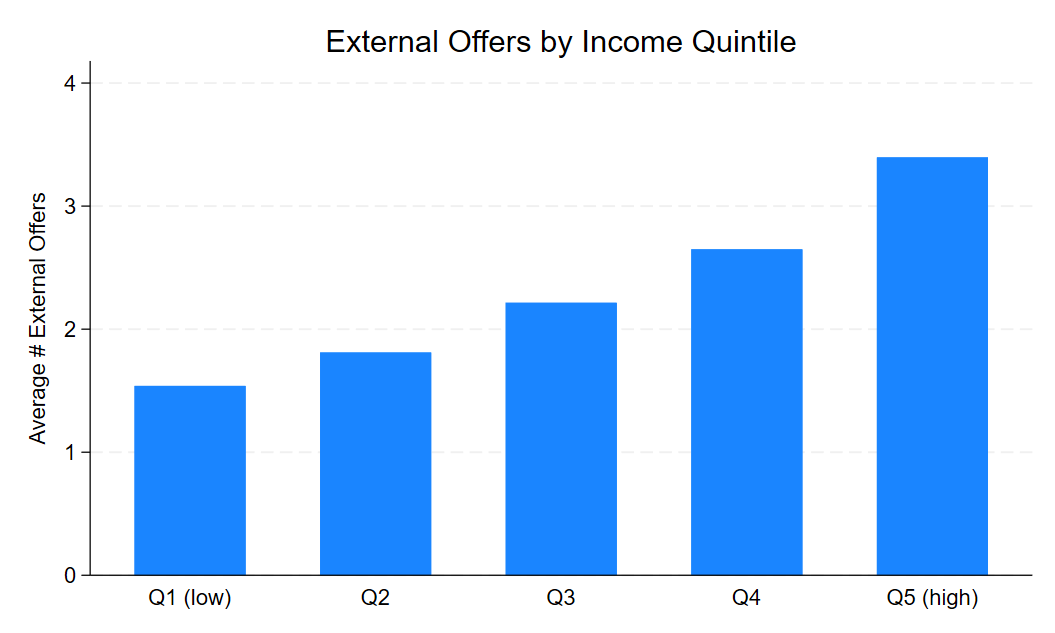
\includegraphics[scale=0.27]{figures/IE2_search_by_income_quintile.png}
\end{tabular}
\end{figure}

Figure \ref{fig:ie2_4} shows the CDF and hazard rate of searches grouped by savings quintile. 

\begin{figure}[H] 
\caption{}
\label{fig:ie2_4}
\centering{}%
\begin{tabular}{cc}
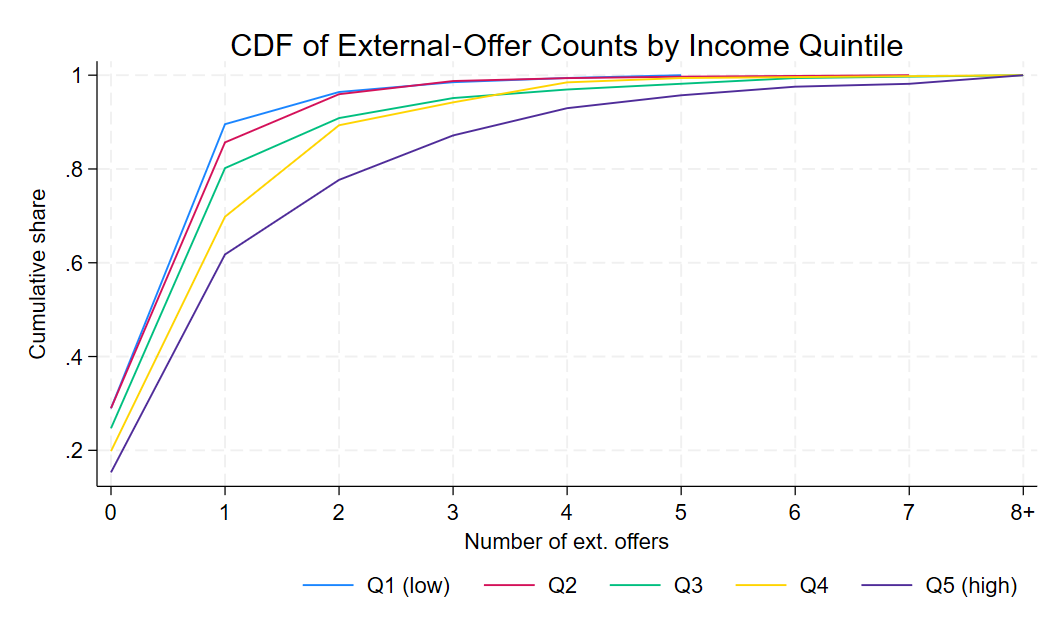
\includegraphics[scale=0.26]{figures/IE2_search_CDF_by_income_quintile.png} & 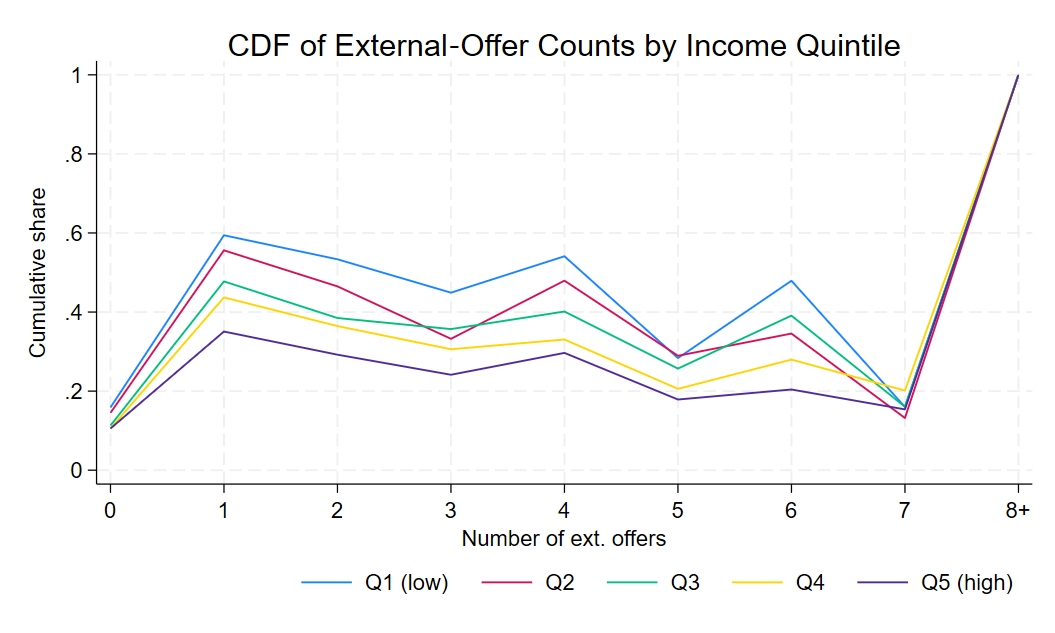
\includegraphics[scale=0.26]{figures/IE2_search_hazardrate_by_income_quintile.png}
\end{tabular}
\end{figure}

\subsection{Dispersion in offers within group}

The insurers in the SCOMP platform observe the age, gender and savings \textcolor{red}{and same zip code?} of the individual. We want to see whether individuals with similar characteristics receive similar offers. 

Given the sparsity of the distribution of individuals it is difficult to find individuals with exactly the same characteristics. Hence we created two criteria to define a group: 
\begin{enumerate}
    \item Individuals within the 5-year age interval, same savings quintile and same gender who receive offers the same year by same firm. we call them group 1  
    \item Indivduals with the same age, gender and savings. who receive offers the same year by same firm. we call them group 2
    \item   Indivduals with the same age, gender and savings. we call them group 3
\end{enumerate}
where the first criteria is less sparse than the second. 
Note that using criteria 1 we could group a man of age 60 and savigs of 954 and and an individual of age 64 and savings of 1089, hence certain dispersion is expected. To reduce the role of savings on the offer dispersion we define the ratio as the savings didivded by the offer. 

Then we studied the dispersion of the offers within each group. 

The following table presents the summary statistics for dispersion variables. 
z\_offer is the percentual dispersion of the offers within groups formed by criteria 1. 
z\_offer2 is the percentual dispersion of the offers within groups formed by criteria 2.
Note that as expected the dispersion in the second case is much lower (.06 against .19) since we are comparing individuals that are more similar. 

In row 3 we show the standard deviation of the offers using criteria 2. The average deviation is .49UF which is around 20USD. This dispersion could be justified by intermediaries, ZIP code, particular day, etc. 

Finally we show the dispersion of our ratio variable using both criteria. As expected the dispersion using criteria 1 decreases significantly since now we are in certain way controling for savings. The dispersion using the criteria 2 does not change much. 


\begin{table}[htbp]\centering
\def\sym#1{\ifmmode^{#1}\else\(^{#1}\)\fi}
\caption{Summary Statistics}
\begin{tabular}{l*{1}{ccccc}}
\hline\hline
            &\multicolumn{5}{c}{(1)}                                         \\
            &\multicolumn{5}{c}{}                                            \\
            &        mean&          sd&         min&         max&       count\\
\hline
z\_offer     &    .1930441&    .1193585&           0&    .9220387&       88324\\
z\_offer2    &    .0651742&    .0525936&           0&    .4111664&       24022\\
sd\_offer2   &    .4973616&    .5770213&           0&    6.349819&       24022\\
z\_ratio     &    .0770126&    .0300375&    .0002599&     .286424&       88324\\
z\_ratio2    &    .0647065&     .052319&           0&    .4111664&       24022\\
\hline
\(N\)       &       88324&            &            &            &            \\
\hline\hline
\end{tabular}
\end{table}


Moreover, if we run a regression of offers on group (using criteria 2) fixed effects, we find that the R2 is .98 meaning that the groups capture almost all the variance in the offers. using criteria 3 the R2 is .99 

\text{In terms of modeling, the previous findings suggest that we can assume that the insurers look at savings, gender and age and send offers based on these characteristics. }


\subsection{dispersion within group for external and internal offers. }


\textcolor{red}{STILL HAVE TO IMPROVE THIS SECTION: HAVEN'T FOUND ANY INTERESTING RESULTS YET}

\subsection{Others}

\subsubsection{Dispersion of the choice set}
Figure \ref{fig:ie2_5} shows the distribution of standard deviations of the choice set of the consumers and the left panel shows the distribution of the range, both of them normalized by the mean of the offers each individual receives.  The table below shows the summary statistics of both variables. Offers have an average deviation from the mean of the offers that represenet a 1.6\% of the mean offer and the range represent a 5.5\% of the mean offer. Considering that this are the savings of their lifetime, this differences translate into considerable absolute differences.
\begin{figure}[H] 
\caption{}
\label{fig:ie2_5}
\centering{}%
\begin{tabular}{cc}
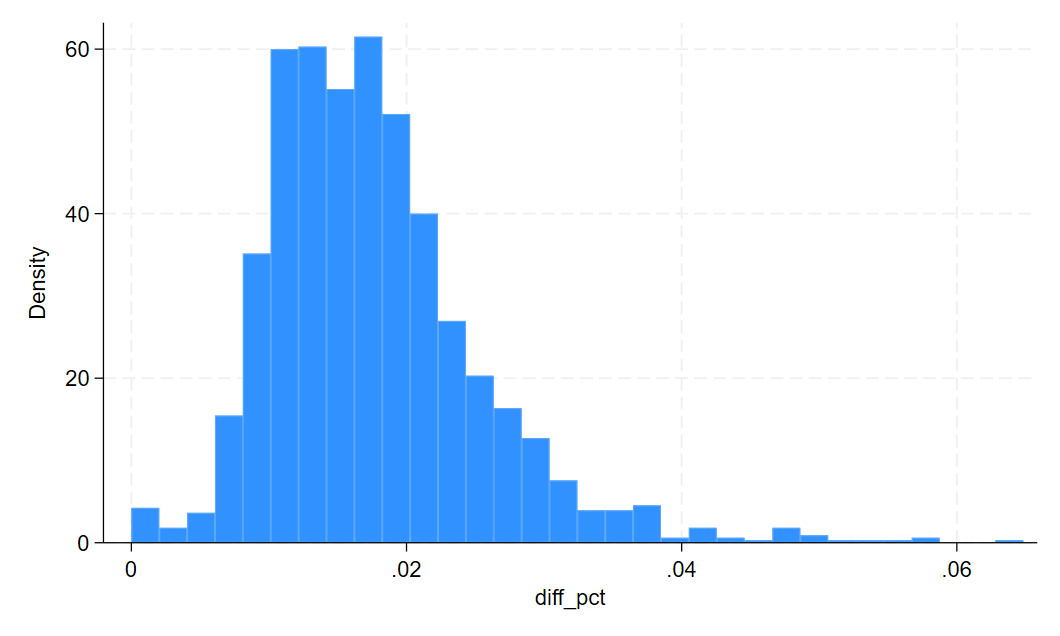
\includegraphics[scale=0.26]{figures/IE2_dispertion_choice_set.png} & 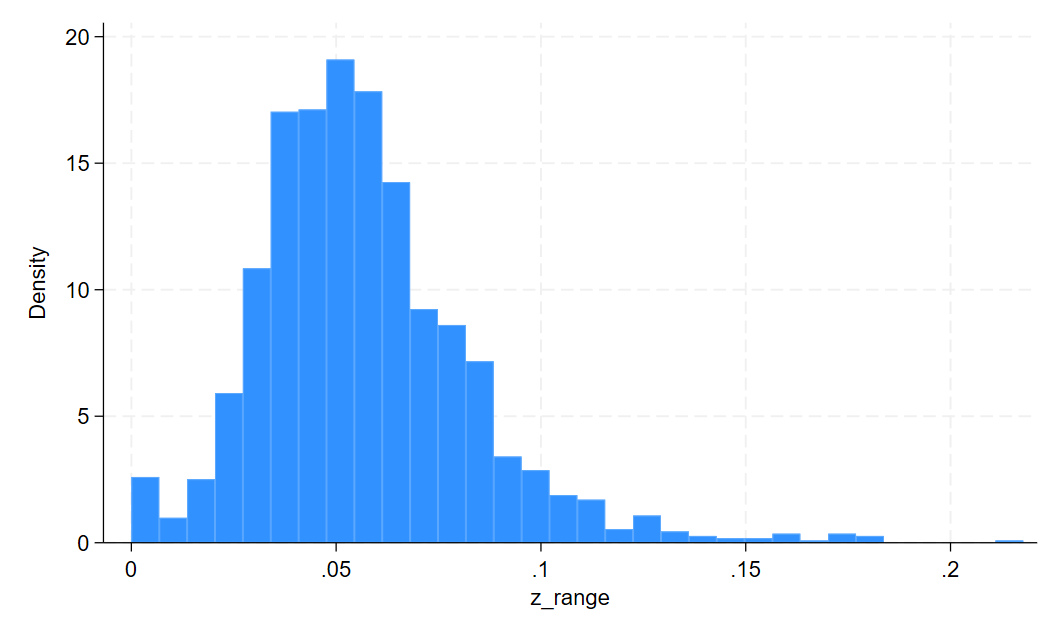
\includegraphics[scale=0.26]{figures/IE2_dispertion_choice_set_range.png}
\end{tabular}
\end{figure}



\begin{table}[htbp]\centering
\def\sym#1{\ifmmode^{#1}\else\(^{#1}\)\fi}
\caption{Summary Statistics}
\begin{tabular}{l*{1}{ccccc}}
\hline\hline
            &\multicolumn{5}{c}{(1)}                                         \\
            &\multicolumn{5}{c}{}                                            \\
            &        mean&          sd&         min&         max&       count\\
\hline
diff\_pct    &    .0179605&    .0075445&           0&    .0648298&       22739\\
z\_range     &     .060962&    .0258919&           0&    .2177676&       22749\\
\hline
\(N\)       &       22749&            &            &            &            \\
\hline\hline
\end{tabular}
\end{table}



\subsubsection{Improvment when asking for external offers}

\begin{table}[htbp]\centering
\def\sym#1{\ifmmode^{#1}\else\(^{#1}\)\fi}
\caption{Summary Statistics}
\begin{tabular}{l*{1}{ccccc}}
\hline\hline
            &\multicolumn{5}{c}{(1)}                                         \\
            &\multicolumn{5}{c}{}                                            \\
            &        mean&          sd&         min&         max&       count\\
\hline
improvement &    .0172569&    .0132584&    -.025862&    .1528358&        2045\\
\hline
\(N\)       &        2045&            &            &            &            \\
\hline\hline
\end{tabular}
\end{table}






\section{IE 3}

Figure \ref{fig:ie3_0} shows the number of external offers that buyers request and figure \ref{fig:ie3_1} shows the distribution disaggregated by year. 

\begin{figure}[H]
\caption{}
\label{fig:ie3_0}
\centering{}%
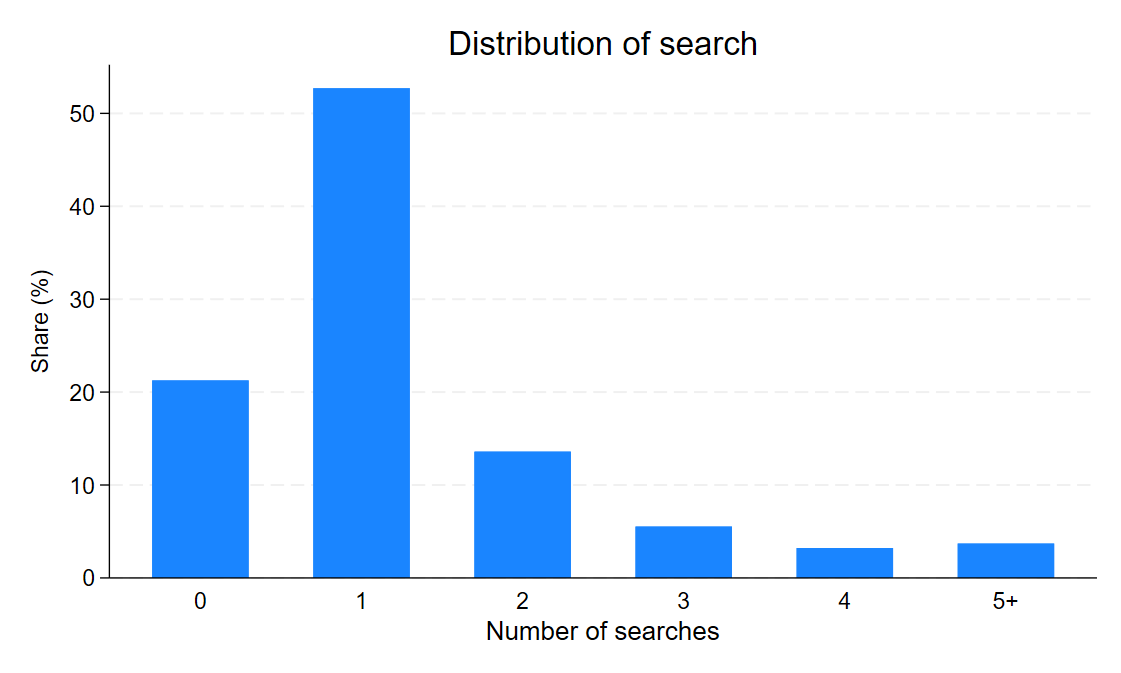
\includegraphics[scale=0.27]{figures/IE3_dist_external_offers.png}
\end{figure}


\begin{figure}[H]
\caption{}
\label{fig:ie3_1}
\centering{}%
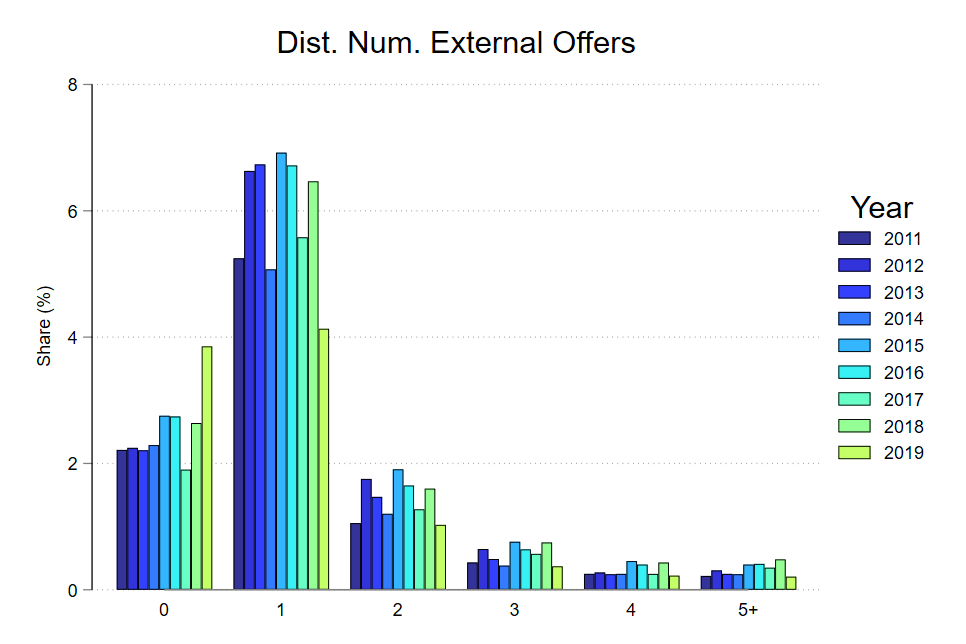
\includegraphics[scale=0.27]{figures/IE3_dist_external_offers_byyear.png}
\end{figure}





Figure \ref{fig:ie3_2} shows 


\begin{figure}[H]
\caption{}
 \label{fig:ie3_2}
\centering{}%
\begin{tabular}{cc}
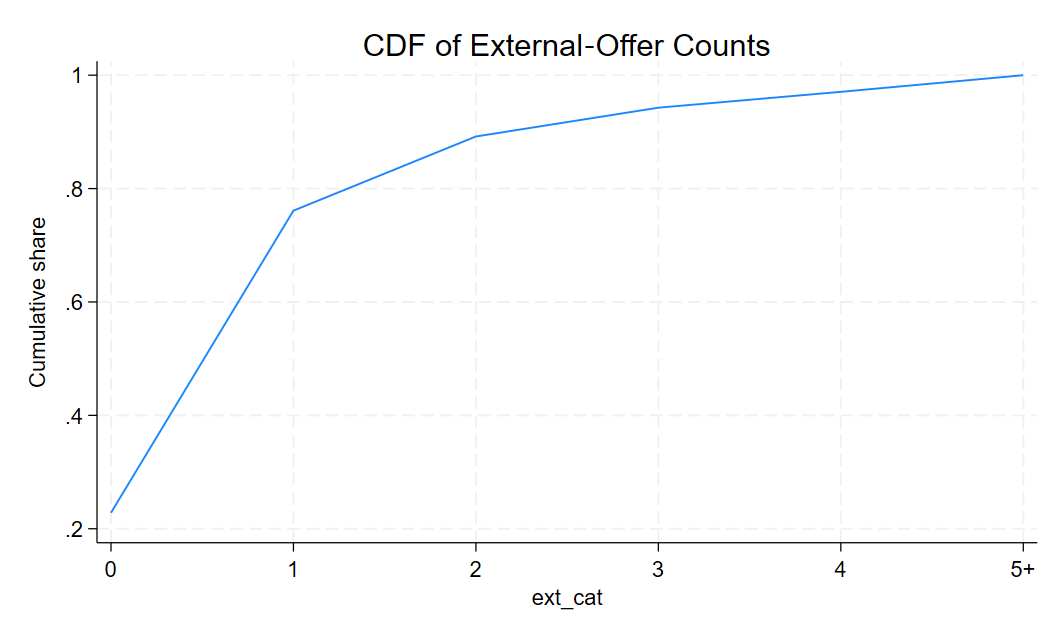
\includegraphics[scale=0.27]{figures/IE3_CDF_number_extoffers.png} &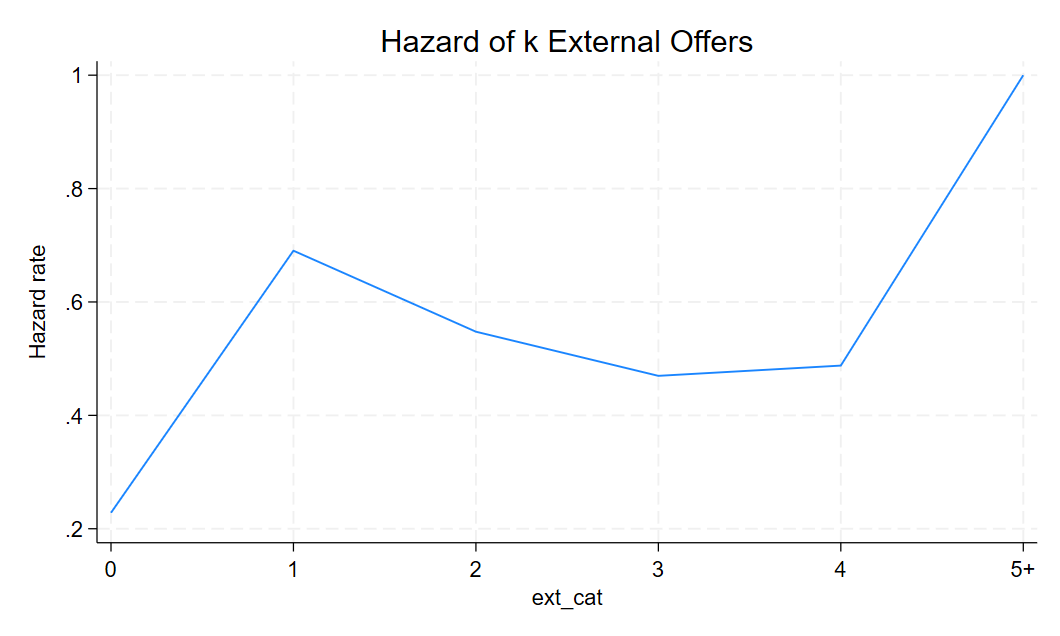
\includegraphics[scale=0.27]{figures/IE3_hazard_number_extoffers.png}
\end{tabular}
\end{figure}



Figure \ref{fig:ie3_3} shows the average number of searches for individuals grouped by their quintile of savings, which is a proxy of income. Specifically an increase of savings by a standard deviation is related to .72 additional searches. 


\begin{figure}[H]
\caption{}
\label{fig:ie3_3}
\centering{}%
\begin{tabular}{cc}
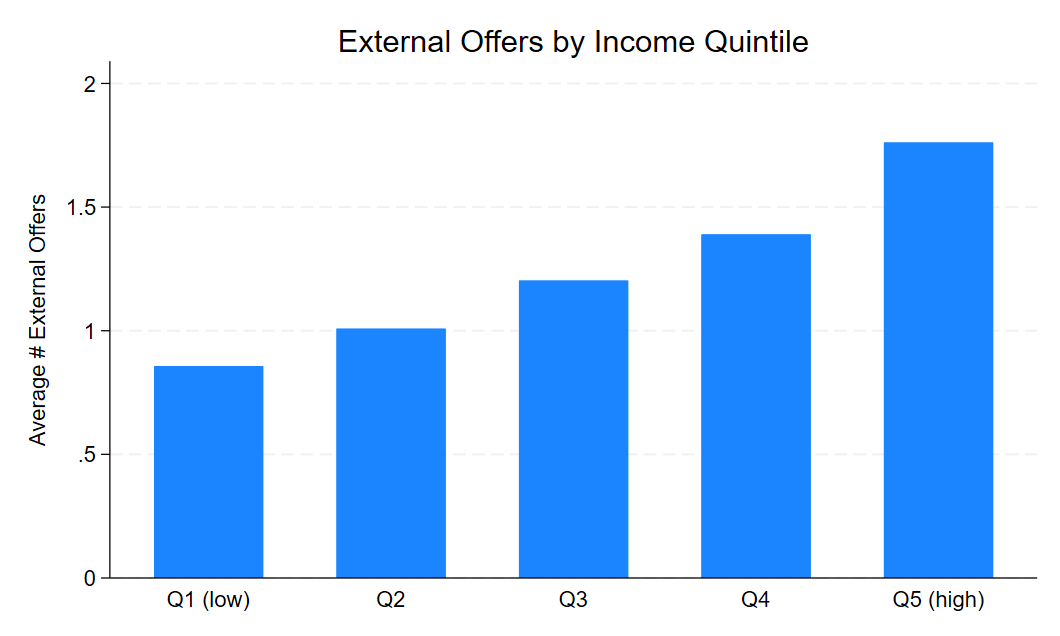
\includegraphics[scale=0.27]{figures/IE3_search_by_income_quintile.png}
\end{tabular}
\end{figure}

Figure \ref{fig:ie3_4} shows the CDF and hazard rate of searches grouped by savings quintile. 

\begin{figure}[H] 
\caption{}
\label{fig:ie3_4}
\centering{}%
\begin{tabular}{cc}
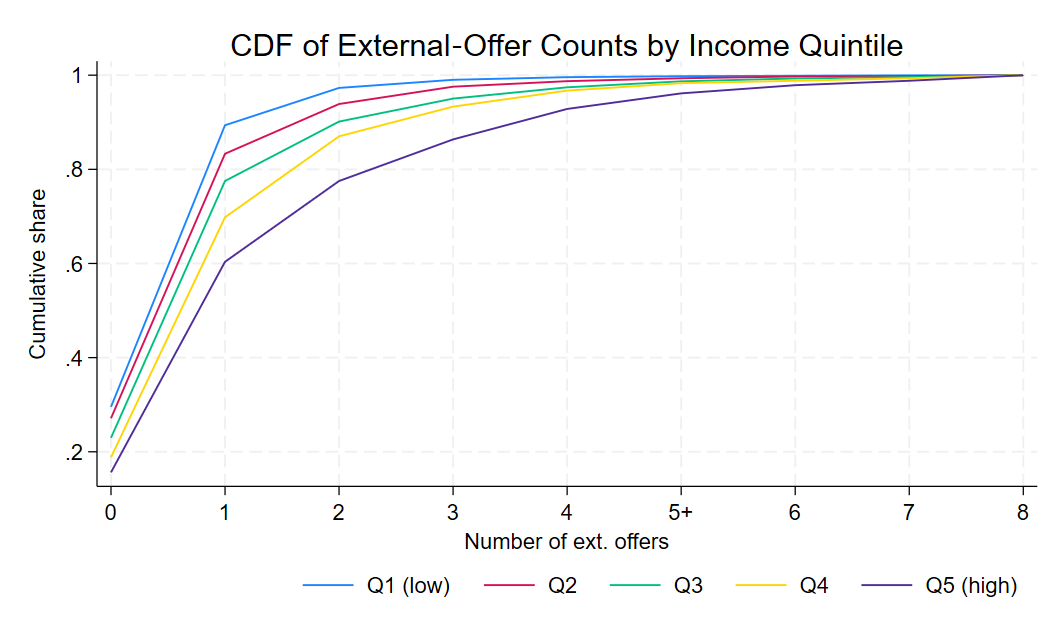
\includegraphics[scale=0.26]{figures/IE3_search_CDF_by_income_quintile.png} & 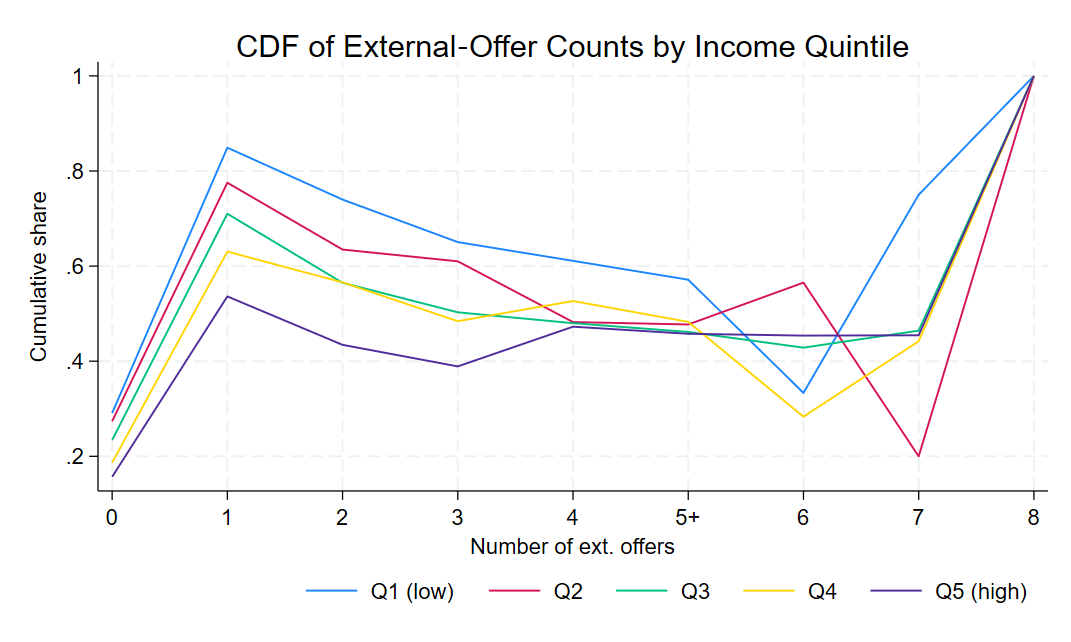
\includegraphics[scale=0.26]{figures/IE3_search_hazardrate_by_income_quintile.png}
\end{tabular}
\end{figure}

\subsection{Dispersion in offers within group}

The insurers in the SCOMP platform observe the age, gender and savings \textcolor{red}{and same zip code?} of the individual. We want to see whether individuals with similar characteristics receive similar offers. 

Given the sparsity of the distribution of individuals it is difficult to find individuals with exactly the same characteristics. Hence we created two criteria to define a group: 
\begin{enumerate}
    \item Individuals within the 5-year age interval, same savings quintile and same gender who receive offers the same year by same firm. we call them group 1  
    \item Indivduals with the same age, gender and savings. who receive offers the same year by same firm. we call them group 2
    \item   Indivduals with the same age, gender and savings. we call them group 3
\end{enumerate}
where the first criteria is less sparse than the second. 
Note that using criteria 1 we could group a man of age 60 and savigs of 954 and and an individual of age 64 and savings of 1089, hence certain dispersion is expected. To reduce the role of savings on the offer dispersion we define the ratio as the savings didivded by the offer. 

Then we studied the dispersion of the offers within each group. 

The following table presents the summary statistics for dispersion variables. 
z\_offer is the percentual dispersion of the offers within groups formed by criteria 1. 
z\_offer2 is the percentual dispersion of the offers within groups formed by criteria 2.
Note that as expected the dispersion in the second case is much lower (.06 against .19) since we are comparing individuals that are more similar. 

In row 3 we show the standard deviation of the offers using criteria 2. The average deviation is .49UF which is around 20USD. This dispersion could be justified by intermediaries, ZIP code, particular day, etc. 

Finally we show the dispersion of our ratio variable using both criteria. As expected the dispersion using criteria 1 decreases significantly since now we are in certain way controling for savings. The dispersion using the criteria 2 does not change much. 


\begin{table}[htbp]\centering
\def\sym#1{\ifmmode^{#1}\else\(^{#1}\)\fi}
\caption{Summary Statistics}
\begin{tabular}{l*{1}{ccccc}}
\hline\hline
            &\multicolumn{5}{c}{(1)}                                         \\
            &\multicolumn{5}{c}{}                                            \\
            &        mean&          sd&         min&         max&       count\\
\hline
z\_offer     &    .1991379&    .1166944&           0&    .8129947&      173923\\
z\_offer2    &    .1205333&    .0795119&           0&    .8659106&      171572\\
z\_offer3    &    .0638504&    .0510833&           0&    .3931563&       60530\\
sd\_offer3   &    .5127416&    .5968534&           0&    10.04091&       60530\\
\hline
\(N\)       &      173964&            &            &            &            \\
\hline\hline
\end{tabular}
\end{table}


Moreover, if we run a regression of offers on group (using criteria 2) fixed effects, we find that the R2 is .98 meaning that the groups capture almost all the variance in the offers. using criteria 3 the R2 is .99 

\text{In terms of modeling, the previous findings suggest that we can assume that the insurers look at savings, gender and age and send offers based on these characteristics. }


\subsection{dispersion within group for external and internal offers. }


\textcolor{red}{STILL HAVE TO IMPROVE THIS SECTION: HAVEN'T FOUND ANY INTERESTING RESULTS YET}

\subsection{Others}

\subsubsection{Dispersion of the choice set}
Figure \ref{fig:ie3_5} shows the distribution of standard deviations of the choice set of the consumers and the left panel shows the distribution of the range, both of them normalized by the mean of the offers each individual receives.  The table below shows the summary statistics of both variables. Offers have an average deviation from the mean of the offers that represenet a 1.6\% of the mean offer and the range represent a 5.5\% of the mean offer. Considering that this are the savings of their lifetime, this differences translate into considerable absolute differences.
\begin{figure}[H] 
\caption{}
\label{fig:ie3_5}
\centering{}%
\begin{tabular}{cc}
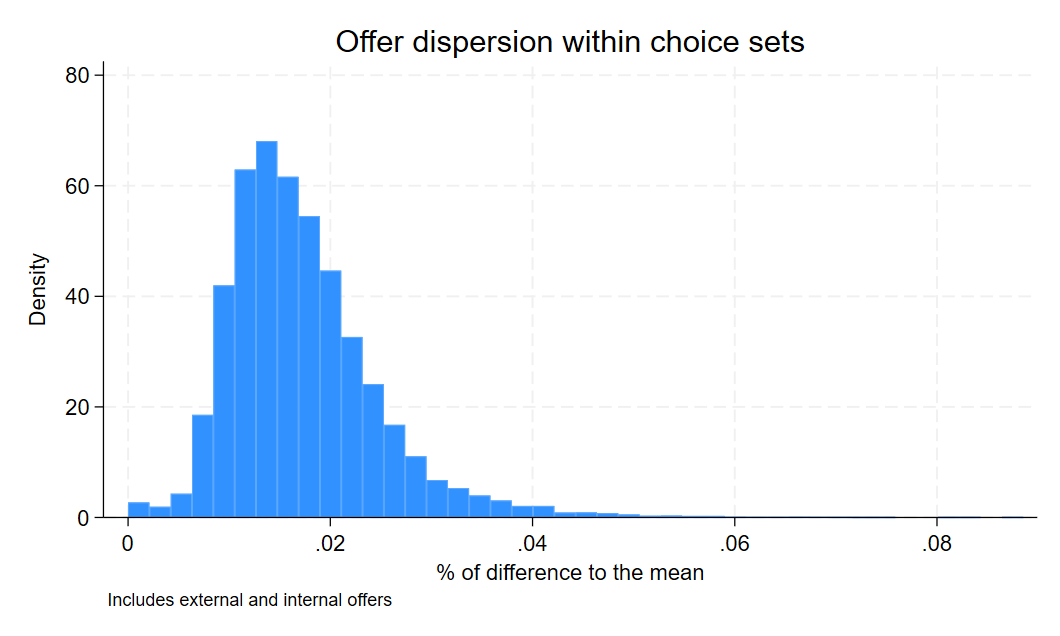
\includegraphics[scale=0.26]{figures/IE3_dispertion_choice_set.png} & 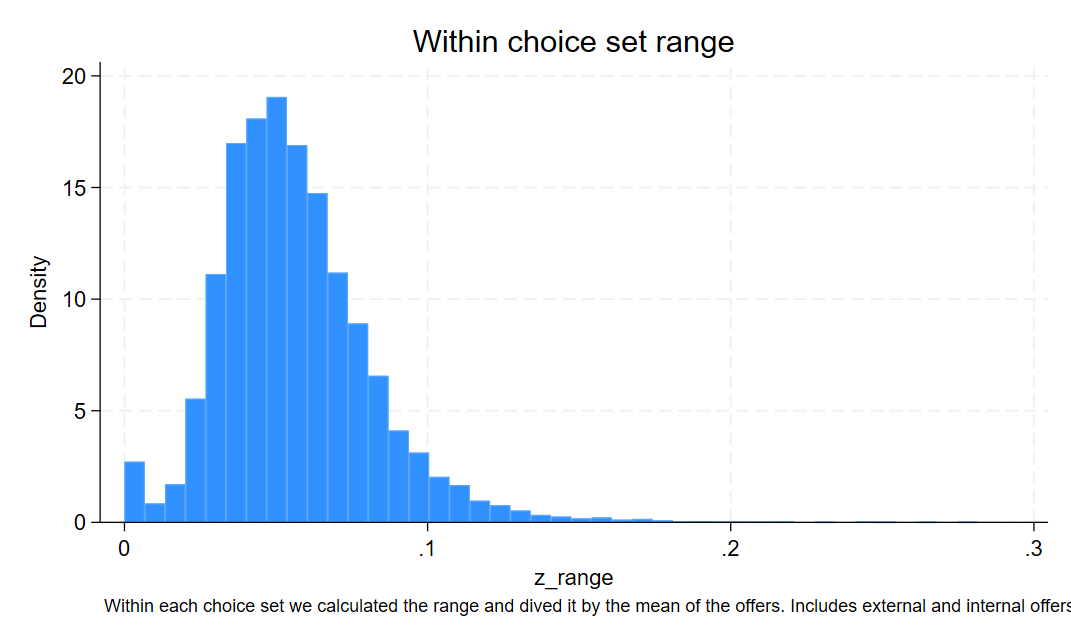
\includegraphics[scale=0.26]{figures/IE3_dispertion_choice_set_range.png}
\end{tabular}
\end{figure}


\begin{table}[htbp]\centering
\def\sym#1{\ifmmode^{#1}\else\(^{#1}\)\fi}
\caption{Summary Statistics}
\begin{tabular}{l*{1}{ccccc}}
\hline\hline
            &\multicolumn{5}{c}{(1)}                                         \\
            &\multicolumn{5}{c}{}                                            \\
            &        mean&          sd&         min&         max&       count\\
\hline
diff\_pct    &    .0176062&    .0072376&           0&    .0909576&      253280\\
z\_range     &    .0602848&    .0249717&           0&     .281407&      253468\\
\hline
\(N\)       &      253468&            &            &            &            \\
\hline\hline
\end{tabular}
\end{table}



\subsubsection{Improvment when asking for external offers}

\begin{table}[htbp]\centering
\def\sym#1{\ifmmode^{#1}\else\(^{#1}\)\fi}
\caption{Improvement when searching}
\begin{tabular}{l*{1}{ccccc}}
\hline\hline
            &\multicolumn{5}{c}{(1)}                                         \\
            &\multicolumn{5}{c}{}                                            \\
            &        mean&          sd&         min&         max&       count\\
\hline
improvement\_abs&    .2429171&    .2865748&   -.6700001&    9.050003&       19142\\
improvement\_pct&    1.763955&    1.303467&   -10.48513&    15.43956&       19142\\
improvement\_PV20&    41.51639&    48.97782&   -114.5081&    1546.714&       19142\\
improvement\_wage&    3.922188&    35.43327&   -2.413689&    2802.884&       19038\\
\hline
\(N\)       &       19142&            &            &            &            \\
\hline\hline
\end{tabular}
\end{table}






\end{document}